\documentclass[11pt, a4paper]{article}

\usepackage{graphicx}
\usepackage[english]{babel}
\usepackage[utf8x]{inputenc}
\usepackage{amsmath}

\usepackage[a4paper,top=3cm,bottom=2cm,left=2cm,right=2cm,marginparwidth=1.75cm]{geometry}
\graphicspath{ {./images} }

\begin{document}


\section{Lecture 1 (10/02/2020)}
\subsection{The basics}
In general any dynamics problem is solved in three steps. The first and last of these is not unlike the problems
one would solve in statics. The second step is however new to dynamics.
\begin{description}
    \item[First]  Draw a Free Body Diagram of the problem
    \item[Second] Set up equations of motion, Note that $\Sigma F \neq 0$, instead $\Sigma F = ma$ ($a$ can still be 0)
    \item[Third]  Check if there are enough equations of motion to solve for all unknown variables.
\end{description}
Notation for acceleration, velocity and displacement may vary depending
on personal preference. $\ddot{x}$ is used as a means of writing acceleration
and $\dot{x}$ is used in place of velocity. A single dot is defined as a single derrivative
with respect to time, two dots in turn refers to the second derrivative with respect to time.
\begin{gather*}
    a = \dot{v} = \ddot{x} \\
    v = \dot{x}
\end{gather*}


\subsection{An example problem}
Below will be an example problem of a single cup on an angled plane. The angle between the x-axis
and the plane shall be called $\theta$. Our coordinate system will consist of 2 axes, an $u$- and $v$-axis, 
where $u$ is parallel to the plane and $v$ perpendicular to the plane. See figure 1 for a free body diagram of
the problem. Friction will be ignored for this problem.

\begin{figure}[h]
    \centerline{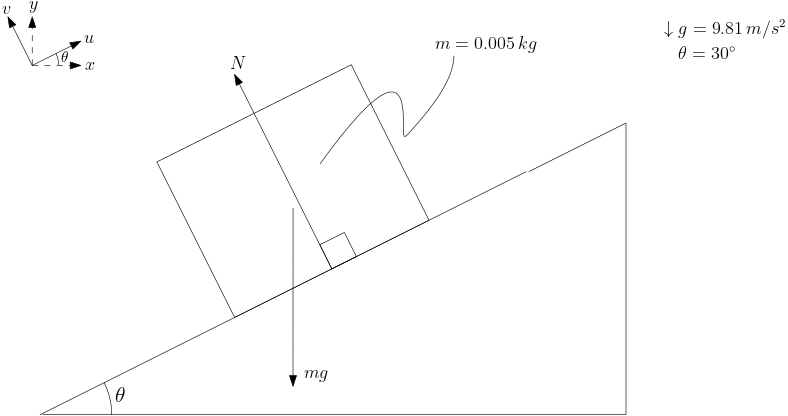
\includegraphics[width=10cm]{images/Crate_No_Friction.png}}
    \caption{The Free Body Diagram of the cup on a plane}
\end{figure}

\begin{gather}
    \Sigma F_u = mg \,\sin(\theta) = m\ddot{u} \\
    \Sigma F_v = N - mg \, \cos(\theta) = m\ddot{v} \\
    \ddot{v} = 0
\end{gather}
Note that equation (3) is typically called a "Constrain Equation"\\
\\
Subsituting equation (3) into (2) will give:
\begin{equation}
    N = m g \,cos(\theta)
\end{equation}
Subsituting equation (4) into (1) and solving for $\ddot{u}$:
\begin{equation}
    \ddot{u} = g \cdot \sin(\theta) = a_u = 4,91 \,m/s^2
\end{equation}
Equation (5) is often (and much to the annoyance of mathematicians) referred to as the "differetial equation".
This equation can be used to determine the velocity and displacement as a function of time. The initial
conditions for this problem will be $x_0 = 0$ and $v_0 = 0$.
\begin{gather}
    \dot{u} = \int \ddot{u} \,dt = a_u t + C_1\\
    \dot{u}(0) = 0\,m/s \quad \rightarrow \quad C_1 = 0 \notag \\
    u = \int \dot{u} \,dt = \int a_u t \,dt = \frac{1}{2} a_u t^2 + C_2\\
    u(0) = 0\,m \quad \rightarrow \quad C_2 = 0 \notag
\end{gather}
thus when subsituting in equation (5) in (6) and (7) the final answer becomes:
\begin{gather*}
    \dot{u} = 4,91 \cdot t \\
    u = \frac{1}{2} \cdot 4,91 \cdot t^2
\end{gather*}


\subsection{Friction with an example}
\setcounter{equation}{0}
The equation for kinetic friction is much the same as the equation
for static friction with a few key differences. Note that in general $\mu_k < \mu_s$.
\begin{gather*}
    F_w = \mu_k N \\
    F_w \leq \mu_s N
\end{gather*}
Solving a dynamics problem involving frictional forces, forces us to make an assumption
at some point. Either the object is moving in which case dry friction does occur,
or the object is in static equilibrium in which case the acceleration parallel to the plane will be zero.

\begin{figure}[h]
    \centerline{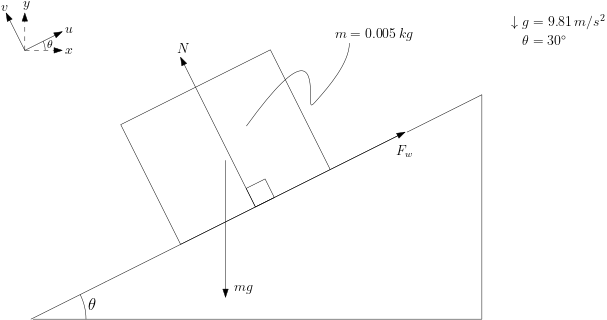
\includegraphics[width=10cm]{images/Crate_Friction.png}}
    \caption{The Free Body Diagram of the cup on a plane}
\end{figure}

\begin{gather}
    \Sigma F_u = -F_w + mg \, \sin(\theta) = m\ddot{u}\\
    \Sigma F_v = N - mg \, \cos(\theta) = m\ddot{v}\\
    \ddot{v} = 0
\end{gather}
This is the point where we assume whether dry friction will or will not occur. For this example
both assumptions will be shown.
\newpage

\underline{Dry Friction does not occur:}\\
\begin{gather}
    \ddot{u} = 0 \\
    F_w \leq \mu_s N
\end{gather}
the object must be in static equilibrium since dry friction does not occur. In this case
an extra constraint equation is introduced to the system. Solving the system with
$\ddot{u}=0$ will give a value for $F_w$ which should be filled in equation
(5) to make sure the assumption was correct. If the inequality holds the assumption
was correct.\\
\\

\setcounter{equation}{3}
\underline{Dry friction does occur:}\\
\begin{equation}
    F_w = \mu_k N
\end{equation}
In case dry friction does occur the object is sliding across a surface. In this
case the object is sliding down the plane. After solving for the value of $\ddot{u}$ it
should be checked for direction. If the direction is sliding down the plane like we
would expect due to gravity excisting the assumption holds. If the direction is opposite
to the expected direction the assumption was false. This would imply the object is magically 
sliding upwards across the surface due to friction. This does not make sense due to the fact
that friction always is a reactionary force rather then an external one. 


\subsection{Applications of calculus}
Calculus is among one of the most important tools for any problem involving a dynamical system.
In general the posistion and velocity of any system can be described by integration of the "differential equation"
that follows from solving the equations of motion. Vice versa differentiation can be used to determin
the acceleration, and by extension the forces acting on a given particle or body. The most
important aspects of describing motion with calculus will be listed below. Note that all of these are time dependent.

\begin{gather*}
\ddot{x} = \frac{d\dot{x}}{dt} \quad \text{or} \quad a = \frac{dv}{dt}  \\
\ddot{x} = \frac{d^2x}{dt^2} \quad \text{or} \quad a = \frac{d^2x}{dt^2} \\
\dot{x} = \frac{dx}{dt} \quad \text{or} \quad v = \frac{dx}{dt}\\
\dot{x} = \int \ddot{x} \,dt \quad \text{or} \quad v = \int a \,dt\\
x = \int \dot{x} \,dt \quad \text{or} \quad x = \int v \,dt
\end{gather*}


\end{document}